%---------------------------------------------------------------------------------------------------
\chapter{Gravity as Geometry}
\label{chap:gravity}
%---------------------------------------------------------------------------------------------------

\glsunset{GR}
In this chapter, we will introduce and briefly explore different geometrical objects, curvature, torsion and non-metricity, that we use to formulate different theories of gravity, some of which are equivalent to \gls{GR}.
\glsreset{GR}


%---------------------------------------------------------------------------------------------------
\section{Geometrical Objects}
\label{sec:geometrical-objects}
%---------------------------------------------------------------------------------------------------

It is known that a spacetime is endowed with two objects that, in principle, are independent from each other \cite{Inverno}. Those objects are the metric, a rank 2 covariant tensor field which written generically as $g_{\mu \nu}$, that is used in order to define lengths and angles. The other object, referred to as the affine connection and represented symbolically by $\Gamma^\lambda{}_{\mu \nu}$, will allow us to speak of parallel transport and to define the covariant derivative.

In order to speak of lengths we introduce the square of an infinitesimal displacement between two points, $ds^2$, which is known as ``line element'' and is given by

\begin{equation}
    ds^2 = g_{\mu \nu} dx^\mu dx^\nu \,.
\end{equation}
Even though the metric tensor depends on the coordinates of spacetime, we will not make explicit reference to it, leaving the dependency implicit. The metric is used to define the length of a contravariant vector $V^\mu$ as

\begin{equation}
    V^2 = g_{\mu \nu} V^\mu V^\nu \,.
\end{equation}
The metric will also allow us to speak of angles between two contravariant vectors, where the cosine between the vector $V^\mu$ and the vector $U^\nu$ is

\begin{equation}
    cos(V, U) = \frac{g_{\mu \nu} V^\mu U^\nu}{\sqrt{g_{\mu \nu} V^\mu V^\nu g_{\rho \sigma} U^\rho U^\sigma}} \,.
\end{equation}
Finally, for a non-singular metric, that is a metric where its determinant $g \equiv det(g_{\mu \nu})$ is non zero, the inverse of $g_{\mu \nu}$ is given by $g^{\mu \nu}$ such that

\begin{equation}
    g_{\alpha \nu} g^{\nu \beta} = \delta^\beta_\alpha \,.
\end{equation}
The metric and its inverse allow us to raise and lower indices on other quantities, e.g. $V_\mu = g_{\mu \nu} V^\nu$.

Unlike what happens in an Euclidean geometry, in a curved spacetime two nearby points might not necessarily share the same tangent space, which means that it is not possible to define parallel transport in the usual way. We can introduce the affine connection, $\Gamma^\mu{}_{\alpha \beta}$, to relate two nearby tangent spaces by assuming that the displacement is bilinear with both the contravariant vector, which is being propagated, and the displacement. Formally, if we take a contravariant vector $V^a(x)$ and transport it in parallel to $x + \delta x$, $\tilde{V}^a(x + \delta x)$, we can relate the two with

\begin{equation}
    V^\mu(x) - \tilde{V}^\mu (x + \delta x) = \Gamma^\mu{}_{\alpha \beta} V^\alpha (x) \delta x^\beta \,.
\end{equation}

\noindent Computing the limit when the displacement goes to zero, allow us to define the covariant derivative as
\begin{equation}
    \nabla_\mu V^\nu \equiv \partial_\mu V^\nu + \Gamma^\nu{}_{\alpha \mu} V^\alpha \,,
\end{equation}
Where $\partial_\mu \equiv \partial/\partial x^\mu$ is the partial derivative with respect to the coordinate $x^\mu$. If we assume that the covariant derivative has to obey the Leibniz rule, it follows that for a covariant vector

\begin{equation}
    \nabla_\mu V_\nu = \partial_\mu V^\nu - \Gamma^\alpha{}_{\nu \mu} V_\alpha \,.
\end{equation}

By contrast to what happens with partial derivatives, if we apply two successive covariant derivatives to a vector, it does not, in general, give the same result as when the order of the derivatives is reversed. That is to say that, in general, the commutator does not vanish, and is given by

\begin{equation}
    [\nabla_\mu, \nabla_\nu] V^\alpha = R^\alpha{}_{\beta \mu \nu} V^\beta + T^\sigma{}_{\mu \nu} \nabla_\sigma V^\alpha \,,
\end{equation}
where we introduce the Riemann tensor as

\begin{equation}
    \label{eq:riemann}
    R^{\sigma}{}_{\rho\mu\nu} \equiv
    \partial_{\mu} \Gamma^{\sigma}{}_{\nu\rho} - \partial_{\nu} \Gamma^{\sigma}{}_{\mu\rho} + \Gamma^{\alpha}{}_{\nu\rho} \Gamma^{\sigma}{}_{\mu\alpha} -
    \Gamma^{\alpha}{}_{\mu\rho} \Gamma^{\sigma}{}_{\nu\alpha} \,.
\end{equation}
and the torsion, which encodes the asymmetric part of the affine connection, defined as

\begin{equation}
    T^\lambda{}_{\mu \nu} \equiv \Gamma^\lambda{}_{\mu \nu} - \Gamma^\lambda{}_{\nu \mu} \,.
\end{equation}

Generically, the metric and the affine connection are independent from each other. One can decompose the affine connection as a sum of three different contributions \cite{GeneralizationsGR-R2018}

\begin{equation}
    \label{eq:affine-connection}
    \Gamma^{\lambda}{}_{\mu\nu} =
    \left\lbrace {}^{\lambda}{}_{\mu\nu} \right\rbrace +
    K^{\lambda}{}_{\mu\nu} +
    L^{\lambda}{}_{\mu\nu} \,,
\end{equation}
where the first term is the Levi-Civita connection, depending only on the metric and its derivatives, which is defined as

\begin{equation}
    \left\lbrace {}^{\lambda}{}_{\mu \nu} \right\rbrace \equiv
    \frac{1}{2} g^{\lambda \beta}
    \left( \partial_{\mu} g_{\beta\nu} + \partial_{\nu} g_{\beta\mu} -
    \partial_{\beta} g_{\mu\nu} \right) \,,
\end{equation}
the second term is referred to as the contortion, which is defined as

\begin{equation}
    K^{\lambda}{}_{\mu\nu} \equiv \frac{1}{2} g^{\lambda \beta}
    \left( T_{\mu\beta\nu} + T_{\nu\beta\mu} + T_{\beta\mu\nu} \right) \,,
\end{equation}
and the third object is referred to as disformation, which is defined by

\begin{equation}
    L^{\lambda}{}_{\mu\nu} \equiv \frac{1}{2} g^{\lambda \beta}
    \left( -Q_{\mu \beta\nu}-Q_{\nu \beta\mu}+Q_{\beta \mu \nu} \right) \,.
\end{equation}

It is possible to see that the contortion includes all the contributions coming from the torsion tensor, whereas disformation encodes all of the contributions coming from the existence of non-metricity, that is, the covariant derivative of the metric, which is formally defined as

\begin{equation}
    Q_{\alpha \mu \nu} \equiv \nabla_\alpha g_{\mu \nu} =
    \partial_\alpha g_{\mu \nu} - \Gamma^\beta{}_{\alpha \mu} g_{\beta \nu} - \Gamma^\beta{}_{\alpha \nu} g_{\mu \beta} \,.
\end{equation}

Each of the previously defined geometrical objects, that is, curvature, torsion and non-metricity, have a unique and distinct effect on the propagation of vectors in spacetime. It is in fact possible to provide some geometrical intuition behind each geometrical object, which we represent diagrammatically in \cref{fig:geometrical-interpretation}, and summarize as follows \cite{Jimenez2019a}:

\begin{itemize}
    \item Curvature: Measures the rotation experienced by a vector when subject to parallel transport along a closed curve;
    \item Torsion: Measures the non-closure of the parallelogram when two infinitesimal vectors are subject to parallel transport along each other;
    \item Non-metricity: Measures how much of the length of the vector changes when subject to parallel transported along any given curve.
\end{itemize}

\begin{figure}[h!]
    \centering
    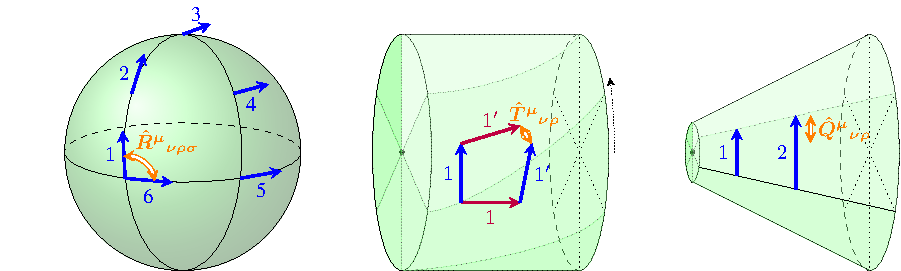
\includegraphics{figures/geometrical-interpretation.pdf}
    \caption
    [Diagrammatic representation of the effect of curvature, torsion and non-metricity on a vector when subject to parallel transport]
    {Diagrammatic representation of the effect of curvature, torsion and non-metricity on a vector when subject to parallel transport. Taken from \cite{Teleparallel-R2021}}
    \label{fig:geometrical-interpretation}
\end{figure}

In order to construct a theory of gravity, one is required to choose which geometrical objects are at play in our spacetime. \Gls{GR} singles out the curvature, presented in \cref{eq:riemann}, and assumes $K^\lambda{}_{\mu \nu} = L^\lambda{}_{\mu \nu} = 0$ in \cref{eq:affine-connection}. However, one can choose to work with geometrical objects other than the curvature, allowing us to create theories of gravity that rely on non-metricity or torsion. In fact, we could, in practice, choose two or more objects to fix the underlying geometry, and create theories of gravity which rely on more than one geometrical object. A schematic representation of the different theories of gravity that can be built using the different geometrical objects at stake can be seen in \cref{fig:geometries}.

\begin{figure}[h!]
    \centering
    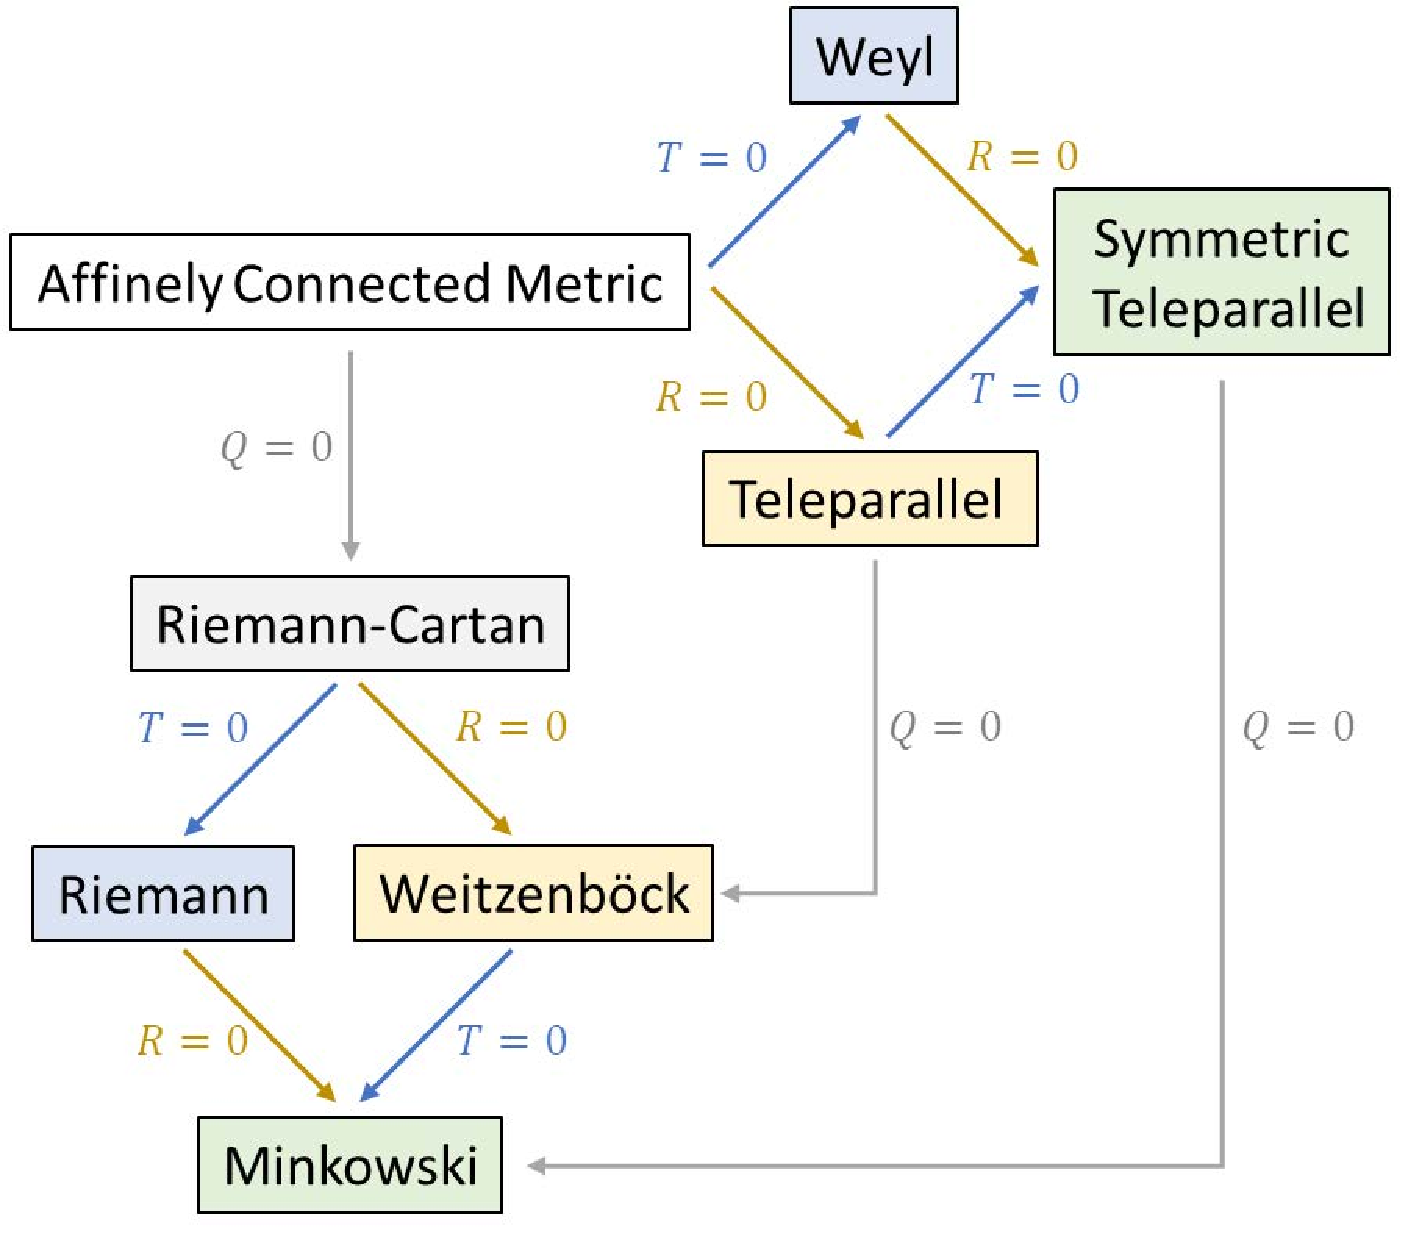
\includegraphics[width=0.6\columnwidth]{figures/geometries.pdf}
    \caption
    [Schematic representation of the different possible spacetime geometries built using curvature, torsion and non-metricity.]
    {Schematic representation of the different possible spacetime geometries built using curvature, torsion and non-metricity. Taken from \cite{Conroy2017}.}
    \label{fig:geometries}
\end{figure}


%---------------------------------------------------------------------------------------------------
\section{The Trinity of Gravity}
%---------------------------------------------------------------------------------------------------

One of the most remarkable consequences of the interplay between the different geometrical objects, is that it is entirely possible to build geometrical theories of gravity which are equivalent to \gls{GR}, but without relying on curvature, and instead making use of either non-metricity or torsion.

To provide a glimpse of this equivalence, we will introduce the notation and ideas that were introduced in \cite{Jaerv2018}. When we are considering a given geometrical object, dependent on the connection, keeping null torsion and null non-metricity, we will label it with an ``LC'' on top of it, to denote it only depends on the contributions coming from the Levi-Civita connection. Similarly, when considering a curvature and non-metricity spacetime, we will use the label ``W'', to denote a Weitzenb$\ddot{\text{o}}$ck geometry. For a geometry with no curvature nor torsion we will use the label ``ST'', which represents the Symmetric Teleparallel setting.

Using the previous notation, one can rewrite the Riemann tensor, presented in \cref{eq:riemann}, by separating the contributions coming from the Levi-Civita connection from the contributions due to torsion and non-metricity. The Riemann tensor now reads

\begin{equation}
    \label{eq:riemann-separated}
    R^{\sigma}{}_{\rho \mu \nu} =
    \overtext{LC}{R}^{\sigma}{}_{\rho \mu \nu} +
    \overtext{LC}{\nabla}_{\mu}  M^{\sigma}{}_{\nu \rho} -
    \overtext{LC}{\nabla}_{\nu}  M^{\sigma}{}_{\mu \rho} +
    M^{\alpha}{}_{\nu \rho} M^{\sigma}{}_{\mu \alpha} -
    M^{\alpha}{}_{\mu \rho} M^{\sigma}{}_{\nu \alpha} \,,
\end{equation}
where $M^\lambda{}_{\mu \nu}$ includes all contributions coming from both torsion and non-metricity, and is defined as

\begin{equation}
    M^\lambda{}_{\mu \nu} \equiv K^\lambda{}_{\mu \nu} + L^\lambda{}_{\mu \nu} \,.
\end{equation}

\noindent Additionally, one can define a tensorial quantity which is known as the Ricci tensor

\begin{equation}
    R_{\mu \nu} = R^\alpha{}_{\mu \alpha \nu} \,,
\end{equation}
that can be used to define the Ricci scalar in the following manner

\begin{equation}
    R \equiv g^{\mu \nu} R_{\mu \nu} \,.
\end{equation}
Computing the value of the Ricci scalar explicitly taking into consideration the form of the Riemann tensor presented in \cref{eq:riemann-separated}, yields

\begin{equation}
    \label{eq:curvature-scalar}
    R = \overtext{LC}{R} + M^{\alpha}{}_{\nu \rho} M^{\mu}{}_{\mu \alpha} g^{\nu \rho} -
    M^{\alpha}{}_{\mu \rho} M^{\mu}{}_{\nu \alpha} g^{\nu \rho} +
    \overtext{LC}{\nabla}_{\mu} \left( M^{\mu}{}_{\nu \rho} g^{\nu \rho}
    - M^{\nu}{}_{\nu \rho} g^{\mu \rho} \right) \,.
\end{equation}

If we restrict the geometry of our spacetime to have vanishing torsion and non-metricity, therefore only including contributions due to curvature, we fall back to the setting of \gls{GR}, where the curvature scalar reduces to the familiar case where

\begin{equation}
    \label{eq:R-RLC}
    R = \overtext{LC}{R} \,.
\end{equation}

In order to have a glimpse of the equivalence, it is useful to remember that it is possible to compute the equations of motion for \gls{GR} by applying the principle of least action to the so called Einstein-Hilbert action

\begin{equation}
    \label{eq:action}
    S = \int \sqrt{-g} \left(  \frac{c^4}{16 \pi G} \overtext{LC}{R} + \mathcal{L}_m \right) dx^4 \,,
\end{equation}
where $g$ is the determinant of the metric $g_{\mu \nu}$ and $\mathcal{L}_m$ is the Lagrangian for the energy-matter content of the universe. We can now obtain the field equations for this theory of gravity by performing the variation of the previous action with respect to the metric. Doing so, one obtains what are the well known \gls{EFE}

\begin{equation}
    \label{eq:EFE}
    \overtext{LC}{R}_{\mu \nu} - \frac{1}{2} \overtext{LC}{R} g_{\mu \nu} = \frac{8 \pi G}{c^4} \mathcal{T}_{\mu \nu} \,,
\end{equation}
where $\mathcal{T}^{\mu \nu}$ is the stress energy tensor

\begin{equation}
    \label{stress-energy-tensor}
    \mathcal{T}^{\mu \nu} \equiv
    \frac{2}{\sqrt{-g}} \frac{\delta (\sqrt{-g} \mathcal{L}_m)}{\partial g_{\mu \nu}} \,.
\end{equation}

If we are to consider a Weitzenb$\ddot{\text{o}}$ck geometry, meaning that we set both non-metricity and curvature to zero, leaving only torsion to play the role of gravity, \cref{eq:curvature-scalar} reduces to

\begin{equation}
    \label{eq:RLC-T}
    \overtext{LC}{R} = -\overtext{W}{T} - 2\overtext{LC}{\nabla}_{\alpha} \overtext{W}{T}^{\alpha} \,,
\end{equation}
where $T$ is the torsion scalar, which is defined in a connection independent manner as

\begin{equation}
    T \equiv \frac{1}{4} T_{\alpha \beta \gamma} T^{\alpha \beta \gamma} +
    \frac{1}{2} T_{\alpha \beta \gamma} T^{\gamma \beta \alpha} -
    T_{\alpha}T^{\alpha} \,,
\end{equation}
and

\begin{equation}
    T_\mu \equiv T^\alpha_{\mu \alpha} \,.
\end{equation}

\noindent By looking at \cref{eq:RLC-T}, we can see that the curvature scalar for \gls{GR} is replaced by the torsion scalar in a Weitzenb$\ddot{\text{o}}$ck geometry plus a divergence term, being acted upon by a covariant derivative. This additional divergence term will be integrated and computed at infinity, i.e. at the boundary, meaning that it does not contribute to the field equations, implying that both of these geometrical settings are equivalent to each other. This geometrical theory of gravity which relies solely on torsion instead of curvature is equivalent to \gls{GR}, and is named the \gls{TEGR}.

Similarly, if we set both the curvature and torsion to zero, leaving non-metricity to mediate the gravitational interaction, the curvature scalar presented in \cref{eq:curvature-scalar} simplifies to

\begin{equation}
    \label{eq:RLC-Q}
    \overtext{LC}{R} = \overtext{ST}{Q} - \overtext{LC}{\nabla}_{\alpha}
    (\overtext{ST}{Q}^{\alpha} - \overtext{ST}{\tilde{Q}}^{\alpha}) \,,
\end{equation}
where $Q$ is the non-metricity scalar that is defined as

\begin{equation}
    \label{eq:Q}
    Q \equiv -\frac{1}{4} Q_{\alpha \beta \gamma} Q^{\alpha \beta \gamma} +
    \frac{1}{2} Q_{\alpha \beta \gamma} Q^{ \gamma \beta \alpha} +
    \frac{1}{4} Q_{\alpha}Q^{\alpha}
    - \frac{1}{2} Q_{\alpha} \tilde{Q}^{\alpha} \,,
\end{equation}
and the two independent contractions of the non-metricity tensor are

\begin{equation}
    Q_\mu \equiv Q_\mu{}^\alpha{}_\mu \,, \hspace{1cm}
    \tilde{Q}^\mu \equiv Q_\alpha{}^{\alpha \mu} \,.
\end{equation}

\noindent By the same arguments that we have used when we had torsion instead of curvature, we can see that the curvature scalar in \cref{eq:RLC-Q} differs only from the non-metricity scalar by a boundary term, implying that this theory is equivalent to \gls{GR}. This non-metric theory of gravity is referred to as the \gls{STEGR}.

The same procedure we have applied in order to obtain the \gls{EFE} can be applied for the case of \gls{STEGR}, where the action will have the non-metricity scalar computed for a flat and torsion-free spacetime, $\overtext{ST}{Q}$, instead of the curvature scalar computed by relying only on the Levi-Civita connection $\overtext{LC}{R}$. Naturally, this also applies for \gls{TEGR}, where the torsion scalar in a metric and flat spacetime $\overtext{W}{T}$ is used instead of $\overtext{LC}{R}$.

The equivalence between these three different theories of gravity, or has it is often referred to as, the three different interpretations of gravity, have been recently popularized as the geometrical trinity of gravity \cite{Jimenez2019a}.


%---------------------------------------------------------------------------------------------------
\section{Generalization of the Trinity of Gravity}
%---------------------------------------------------------------------------------------------------

As we have briefly mentioned in the introduction, the geometrical trinity of gravity is a framework which one can use as a starting point to create modified theories of gravity, knowing that the advancements developed by \gls{GR} will be present.

Although there is a countless number of ways to generalize any given theory, perhaps the most simple way to do so is to promote the scalar quantity in the action for each of the different representations of gravity, to an arbitrary function of itself.

We can apply this procedure to generalize the Einstein-Hilbert action, which leads to the well known and widely studied class of $f(R)$ theories (for a review see e.g.: \cite{Felice2010}). Likewise, one can do the same for a spacetime without curvature and non-metricity, generalizing the \gls{TEGR} to a particular case of \gls{TG}, which we refer to $f(T)$ gravity. This class of theories have also been widely studied, and for a review on the gravity and cosmology behind $f(T)$ we refer the reader to \cite{Teleparallel-R2021}. Of interest to us in this work will be the generalization of \gls{STEGR}, leading us to $f(Q)$ gravity, a particular case of a more general class of theories which are referred to as the \gls{STG}. The action for this theory of gravity reads

\begin{equation}
    \label{eq:f(Q)-action}
    S = \int \sqrt{-g} \left[ -\frac{c^4}{16 \pi G} f(Q) + \mathcal{L}_m \right] d^4x \,.
\end{equation}
When varying the previous action with respect to the metric, one obtains the field equations \cite{Jimenez2019}

\begin{equation}
    \label{eq:f(Q)-field-equations}
    \frac{2}{\sqrt{-g}} \nabla_\alpha \left( \sqrt{-g} f_{Q}(Q) P^{\alpha\mu}{}_\nu \right)
    +  \frac{1}{2} \delta^\mu_\nu f
    +  f_{Q}(Q) P^{\mu\alpha\beta} Q_{\nu\alpha\beta}
    =  \frac{8 \pi G}{c^4} \mathcal{T}^\mu{}_\nu \,,
\end{equation}
where $f_Q(Q) \equiv \partial f(Q) / \partial Q$, $L^\alpha{}_{\mu \nu}$ is the disformation tensor which we have already met previously and $P^{\alpha \mu \nu}$ is the non-metricity conjugate

\begin{equation}
    P^\alpha{}_{\mu \nu} = - \frac{1}{2} L^\alpha{}_{\mu \nu} + \frac{1}{4} (Q^\alpha - \tilde{Q}^\alpha) - \frac{1}{4} \delta^\alpha_{(\mu} Q_{\nu)} \,,
\end{equation}

What is surprising from these generalizations is that, unlike what we expected given the arbitrary nature of the functions $f(Q)$, $f(T)$ and $f(R)$, it is still possible to show that there is a set of assumptions one can make such that the field equations for these theories are the same. In \cite{Boehmer2021} the authors show that under the assumption of a flat, homogeneous and isotropic universe, which is permeated by a perfect fluid, then the field equations derived for $f(Q)$ and $f(T)$ cosmology are formally equivalent, as well as the relationship between the scalar quantity in the action and the Hubble function. Additionally, by decomposing the curvature scalar into the sum of two terms $R = G + B$, where $G$ is a bulk term and $B$ a boundary term, it is also shown that $f(G)$ cosmology is also formally equivalent to the two previous theories. In the spirit of the previous equivalence between geometrical theories this equivalence is, in a sense, a ``cosmological trinity of gravity''. This is of interest to us because, as we will see further ahead in \cref{chap:cosmology}, those are the baseline assumptions for the work developed throughout this dissertation.

An important remark we wish to make is that, due to the lack of coupling between the gravitational sector and the matter content of the universe, these three generalized theories of gravity do not modify the fact that the covariant derivative of the energy-momentum tensor is equal to zero, as shown in \cite{Koivisto2005}.

For the scope of this dissertation, only models based on non-metricity will be considered. To simplify this notation we will often refer to the function $f(Q)$ simplify as $f$ and its derivative as $f_Q$. We will, however, still include explicit dependence on the non-metricity scalar to denote gravitational models based solely on non-metricity, which have an action of the form of the one presented in \cref{eq:f(Q)-action}. Additionally, because curvature and torsion are always set to zero, the label ``ST'' is always assumed to be there on matters of geometry, although no explicit reference to it will be made.
